\documentclass[10pt,a4paper, margin=1in]{article}
\usepackage{fullpage}
\usepackage{amsfonts, amsmath, pifont}
\usepackage{amsthm}
\usepackage{graphicx}
\usepackage{fullpage}
\usepackage{amsfonts, amsmath, pifont}
\usepackage{amsthm}
\usepackage{graphicx}
\usepackage{float}

\usepackage{tkz-euclide}
\usepackage{tikz}
\usepackage{pgfplots}
\pgfplotsset{compat=1.13}
\usepackage[utf8]{inputenc}
\usepackage{geometry}
 \geometry{
 a4paper,
 total={210mm,297mm},
 left=10mm,
 right=10mm,
 top=10mm,
 bottom=16mm,
 } 
 
 % Write both of your names here. Fill exxxxxxx with your ceng mail address.
\author{
  Düzel, Uğur\\
  \texttt{e2171569@ceng.metu.edu.tr}
  \and
  Yalçınkaya, Beyazıt\\
  \texttt{e2172138@ceng.metu.edu.tr}
}
\title{CENG 384 - Signals and Systems for Computer Engineers \\
Spring 2018-2019 \\
Written Assignment 4}
\begin{document}
\maketitle



\noindent\rule{19cm}{1.2pt}

\begin{enumerate}

\item 
	\begin{itemize}
		\item[(a)]
			Below, we give the difference equation of the given system.
			\begin{equation}
				y[n - 2] - 6y[n - 1] + 8y[n] = 16x[n]
			\end{equation}
		
		\item[(b)]
			To find the frequency response of the system, i.e., $H(e^{j\omega})$, we will take the Fourier transform of the system and then use the time shifting property of the discrete-time Fourier transform, i.e., $\mathcal{F}\{x[n - n_0]\} = e^{-j\omega n_0} X(e^{j\omega})$.
			\begin{equation}
			\begin{split}
				e^{-2j\omega } Y(e^{j\omega}) - 6e^{-j\omega } Y(e^{j\omega}) + 8Y(e^{j\omega}) & = 16X(e^{j\omega})\\
				(e^{-2j\omega } - 6e^{-j\omega } + 8)Y(e^{j\omega}) & = 16X(e^{j\omega})\\
				H(e^{j\omega}) = \frac{Y(e^{j\omega})}{X(e^{j\omega})} & = \frac{16}{e^{-2j\omega } - 6e^{-j\omega } + 8}\\
				H(e^{j\omega}) & = \frac{16}{(e^{-j\omega} - 4)(e^{-j\omega} - 2)}\\
				H(e^{j\omega}) & = \frac{8}{e^{-j\omega} - 4} - \frac{8}{e^{-j\omega} - 2}
			\end{split}
			\end{equation}
			
		\item[(c)]
			Rewrite the frequency response $H(e^{j\omega})$ as follows.
			\begin{equation}
			\begin{split}
				H(e^{j\omega}) & = \frac{8}{e^{-j\omega} - 4} - \frac{8}{e^{-j\omega} - 2}\\
				H(e^{j\omega}) & = \frac{4}{1 - \left(\frac{1}{2}\right)e^{-j\omega}} - \frac{2}{1 - \left(\frac{1}{4}\right)e^{-j\omega}}
			\end{split}
			\end{equation}
			To find impulse response of the system, we will use the well know property: $\mathcal{F}\{a^nu[n]\} = \frac{1}{1-ae^{-j\omega}}$ for $|a| < 1$.
			\begin{equation}
			\begin{split}
				h[n] & = \left( 4\left( \frac{1}{2} \right)^n - 2\left( \frac{1}{4} \right)^n \right) u[n]\\
				h[n] & = \left( 2^{2 - n} - 2^{1-2n} \right) u[n]
			\end{split}
			\end{equation}
			
		\item[(d)]
			First, we take the Fourier transform of $x[n] = \left( \frac{1}{4} \right)^n u[n]$ by using the formula $\mathcal{F}\{a^nu[n]\} = \frac{1}{1-ae^{-j\omega}}$ for $|a| < 1$.
			\begin{equation}
				\mathcal{F}\left\{\left( \frac{1}{4} \right)^n u[n]\right\} = \frac{1}{1 - \left( \frac{1}{4} \right)e^{j\omega}} = \frac{4}{4 - e^{j\omega}}
			\end{equation}
			We know that $Y(e^{j\omega}) = H(e^{j\omega}) X(e^{j\omega})$; hence, we get the following.
			\begin{equation}
			\begin{split}
				Y(e^{j\omega}) & = H(e^{j\omega}) X(e^{j\omega})\\
				& = \frac{32}{(e^{-j\omega} - 4)(4 - e^{j\omega})} - \frac{32}{(e^{-j\omega} - 2)(4 - e^{j\omega})}\\
				& = \frac{32}{(e^{-j\omega} - 2)(e^{j\omega} - 4)} - \frac{32}{(e^{-j\omega} - 4)^2}\\
				& = \frac{16}{e^{-j\omega} - 4} - \frac{16}{e^{-j\omega} - 2} + \left( \frac{32}{3} \right) \left( \frac{1}{e^{-j\omega} - 4} + \frac{(1 - e^{-j\omega})}{(e^{-j\omega} - 4)^2} \right)\\
				& = (-4)\frac{1}{1 - \frac{1}{4}e^{-j\omega}} + (8)\frac{1}{1 - \frac{1}{2}e^{-j\omega}} + \left( -\frac{8}{3} \right)\frac{1}{1 - \frac{1}{4}e^{-j\omega}} + \left( \frac{2}{3} \right)\frac{(1 - e^{j\omega})}{(1 - \frac{1}{4}e^{-j\omega})^2}
			\end{split}
			\end{equation}
			Now, we will take the inverse Fourier transform of $Y(e^{j\omega})$ by using following pairs: $\mathcal{F}\{a^nu[n]\} = \frac{1}{1-ae^{-j\omega}}$ for $|a| < 1$, $\mathcal{F}\{(n + 1)a^nu[n]\} = \frac{1}{(1-ae^{-j\omega})^2}$ for $|a| < 1$, and $\mathcal{F}\{x[n] - x[n - 1]\} = (1 - e^{-j\omega})X(e^{j\omega})$ for $\mathcal{F}\{x[n]\} = X(e^{j\omega})$.
			\begin{equation}
				y[n] = (-4)\left( \frac{1}{4} \right)^nu[n] + (8)\left( \frac{1}{2} \right)^nu[n] + \left( -\frac{8}{3} \right)\left( \frac{1}{4} \right)^nu[n] + \left( \frac{2}{3} \right) \left( (n + 1)\left( \frac{1}{4} \right)^nu[n] - n\left( \frac{1}{4} \right)^{n-1}u[n - 1] \right)
			\end{equation}
			Since $n\left( \frac{1}{4} \right)^{n-1}u[n - 1]$ is $0$ at $n = 0$, it is equal to $n\left( \frac{1}{4} \right)^{n-1}u[n]$. Then, we rewrite $y[n]$ as follows.
			\begin{equation}
				y[n] = \left( 2^{3 - n} - 2^{-2n} \left( 2n + 6 \right) \right) u[n]
			\end{equation}

	\end{itemize}
	
	\item
		Since two systems are combined in parallel, the overall impulse response of the system is $h[n] = h_1[n] + h_2[n]$. By linearity property of Fourier transform, we can deduce that $H(e^{j\omega}) = H_1(e^{j\omega}) + H_2(e^{j\omega})$. By using the well-known formula $\mathcal{F}\{a^nu[n]\} = \frac{1}{1-ae^{-j\omega}}$ for $|a| < 1$, we can find $H_1(e^{j\omega})$, i.e., $H_1(e^{j\omega}) = \frac{1}{1 - \frac{1}{3}e^{-j\omega}} = \frac{3}{3 - e^{-j\omega}}$. Since $H_2(e^{j\omega}) = H(e^{j\omega}) - H_1(e^{j\omega})$, we can compute $H_2(e^{j\omega})$ as follows.
			\begin{equation}
			\begin{split}
				H_2(e^{j\omega}) & = H(e^{j\omega}) - H_1(e^{j\omega})\\
				& = \frac{5e^{-j\omega} - 12}{e^{-2j\omega} - 7e^{-j\omega} + 12} - \frac{3}{3 - e^{-j\omega}}\\
				& = \frac{8}{e^{-j\omega} - 4} - \frac{3}{e^{-j\omega} - 3} - \frac{3}{3 - e^{-j\omega}}\\
				& = \frac{8}{e^{-j\omega} - 4} + \frac{3}{3 - e^{-j\omega}} - \frac{3}{3 - e^{-j\omega}}\\
				& = \frac{8}{e^{-j\omega} - 4}
			\end{split}
			\end{equation}
		By using the formula $\mathcal{F}\{a^nu[n]\} = \frac{1}{1-ae^{-j\omega}}$ for $|a| < 1$, $h_2[n]$ is as follows.
			\begin{equation}
				h_2[n] = (-2^{1 - 2n})u[n]
			\end{equation}
		
		
	\item
	\begin{itemize}
	\item[(a)]
		Below, we give the Fourier transform of $x(t)$ by using well-know Fourier transform pairs for the sinc function and cosine.
		\begin{equation}
		\begin{split}
			X(j\omega) = \begin{cases}
			1, \ & \text{if} \ |\omega| < 2\pi\\
			\pi\delta(0), \ & \text{if} \ |\omega| = 3\pi\\
			0, \ & \text{otherwise}
						\end{cases}
		\end{split}
		\end{equation}
		Below, we plot $X(j\omega)$.
	
	\begin{center}	
		\begin{tikzpicture}
	           \begin{axis}[
        	  axis lines=middle,
          xlabel={$\omega$},
          ylabel={$X(j\omega)$},
          xtick={-12, -10, ..., 12},
          ytick={0, ..., 4},
          ymin=-1, ymax=4,
          xmin=-12, xmax=12
        ]
			\draw[->] (axis cs:-3*pi,0) -- (axis cs:-3*pi,pi);
			\draw[->] (axis cs:3*pi,0) -- (axis cs:3*pi,pi);
			\draw[-] (axis cs:2*pi,0) -- (axis cs:2*pi,1);
			\draw[-] (axis cs:-2*pi,0) -- (axis cs:-2*pi,1);
			\draw[-] (axis cs:-2*pi,1) -- (axis cs:2*pi,1);
			\end{axis}
		\end{tikzpicture}
		\end{center}
		
		
		\item[(b)]
			Nyquist frequency, i.e., $\omega_M$, of the system is $3\pi$ and Nyquist period is $\frac{2}{3}$.
		
		\item[(c)]
			By sampling theorem, we know that the sampling fruquency shall be more than Nyquist rate, i.e., $\omega_s > 2\omega_M$. Nyquist rate ($2\omega_M$) is two times Nyquist frequency ($\omega_M$); hence, Nyquist rate is $6\pi$. Therefore, we pick $\omega_s = 8\pi$. Then, we have $T = \frac{1}{4}$. From these, below, we find the Fourier transform of $x_p(t)$, i.e., $X_p(j\omega)$.
		\begin{equation}
		\begin{split}
			X_p(j\omega) & = \frac{1}{T} \sum_{k = -\infty}^{+\infty} X(j(\omega - k\omega_s))\\
			& = 4 \sum_{k = -\infty}^{+\infty} X(j(\omega - 8\pi k))
		\end{split}
		\end{equation}
		Below, we plot $X(j\omega)$.
	
	\begin{center}	
		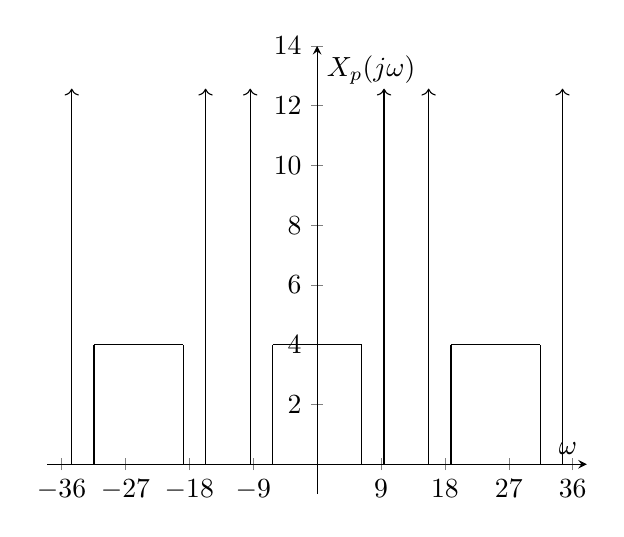
\begin{tikzpicture}
	           \begin{axis}[
        	  axis lines=middle,
          xlabel={$\omega$},
          ylabel={$X_p(j\omega)$},
          xtick={-36, -27, ..., 36},
          ytick={0, 2, 4, ..., 14},
          ymin=-1, ymax=14,
          xmin=-38, xmax=38
        ]
			\draw[->] (axis cs:-3*pi,0) -- (axis cs:-3*pi,4*pi);
			\draw[->] (axis cs:3*pi,0) -- (axis cs:3*pi,4*pi);
			\draw[-] (axis cs:2*pi,0) -- (axis cs:2*pi,4);
			\draw[-] (axis cs:-2*pi,0) -- (axis cs:-2*pi,4);
			\draw[-] (axis cs:-2*pi,4) -- (axis cs:2*pi,4);
			
			\draw[->] (axis cs:5*pi,0) -- (axis cs:5*pi,4*pi);
			\draw[->] (axis cs:11*pi,0) -- (axis cs:11*pi,4*pi);
			\draw[-] (axis cs:10*pi,0) -- (axis cs:10*pi,4);
			\draw[-] (axis cs:6*pi,0) -- (axis cs:6*pi,4);
			\draw[-] (axis cs:6*pi,4) -- (axis cs:10*pi,4);
			
			\draw[->] (axis cs:-11*pi,0) -- (axis cs:-11*pi,4*pi);
			\draw[->] (axis cs:-5*pi,0) -- (axis cs:-5*pi,4*pi);
			\draw[-] (axis cs:-6*pi,0) -- (axis cs:-6*pi,4);
			\draw[-] (axis cs:-10*pi,0) -- (axis cs:-10*pi,4);
			\draw[-] (axis cs:-10*pi,4) -- (axis cs:-6*pi,4);
			\end{axis}
		\end{tikzpicture}
		\end{center}
			
		\end{itemize}
		
	\item
	\begin{itemize}
		\item[(a)]
			Since, $\omega_s = \pi$, $T = 2$. Below, we find $X_d(e^{j\omega})$.
		\begin{equation}
		\begin{split}
			X_d(e^{j\omega}) & = \frac{1}{T} \sum_{k = -\infty}^{+\infty} X_c(j(\omega - 2\pi k)/T)\\
			& = \frac{1}{2} \sum_{k = -\infty}^{+\infty} X_c(j(\omega - 2\pi k)/2)
		\end{split}
		\end{equation}
		We can rewrite $X_d(e^{j\omega})$ as follows.
		\begin{equation}
		\begin{split}
			X_d(e^{j\omega}) = \begin{cases}
			\frac{\omega - 2\pi k}{\pi}, \ & \text{if} \ 2\pi k - \frac{\pi}{2} \leq \omega \leq 2\pi k + \frac{\pi}{2} \ \text{for} \ k = 0, \pm 1, \pm 2, \ldots\\
			0, \ & \text{otherwise}
						\end{cases}
		\end{split}
		\end{equation}
		
		\item[(b)]
			Below, we find the $H(e^{j\omega})$ by using the well-know Fourier transform pair for cosine.
		\begin{equation}
			H(e^{j\omega}) = \pi \sum_{l = -\infty}^{+\infty} \left( \delta(\omega - \pi - 2\pi l) + \delta(\omega + \pi - 2\pi l) \right)
		\end{equation}
		
		\item[(c)]
			By using the multiplication property of discrete-time Fourier transform, we can find $Y_d(e^{j\omega})$ as follows.
		\begin{equation}
		\begin{split}
			Y_d(e^{j\omega}) & = \frac{1}{2\pi} \int_{2\pi} X(e^{j\theta}) H(e^{j(\omega - \theta)})d\theta\\
			& = \frac{1}{2\pi} \int_{-\pi}^{+\pi} X(e^{j\theta}) H(e^{j(\omega - \theta)})d\theta\\
			& = 1
		\end{split}
		\end{equation}
	\end{itemize}
			
  
\end{enumerate}
\end{document}

